\section{Syntax Specification}
\subsection{Reserved words \& Keywords}
In the Ezuino programming language, a reserved keyword is vital to prevent users to overwrite, define and use keywords, which is used in the programming language already. In case that a user tries to define a variable or function named a reserved keyword, they will receive an error, which will be thrown into the error handler. The error handler will then tell the users, where and which reserved keyword they used where. The reserved keywords are words primarily used in the Java and C programming language. The following reserved keywords can be found in figure \ref{rk} below:
\begin{figure}[H]
\centering
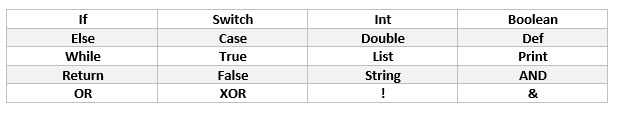
\includegraphics[scale=0.90]{figures/reservedK.png}
\caption{Table of Reserved Keywords}
\label{rk}
\end{figure}

